\section{Dataset Generation Method}
\label{sec:dataset_generation}

In this section, we present our methodology for constructing CVGlobal, a large-scale multi-modal dataset that pairs satellite and street-view imagery across diverse global regions. Our approach systematically samples locations from five continents while ensuring geographical diversity and balanced representation between urban and rural environments.

\subsection{Dataset Design and Sampling Strategy}

Our dataset construction methodology is guided by three key principles: \textit{geographical diversity}, \textit{balanced representation}, and \textit{multi-modal consistency}. We define sampling regions across five major continents (North America, Europe, Asia, South America, and Africa), with each continent contributing equally to the final dataset to prevent geographical bias.

For each continent, we establish two distinct sampling regions:
\begin{itemize}
    \item \textbf{Urban regions}: Areas with high population density and significant urban infrastructure
    \item \textbf{Rural regions}: Areas with low population density and predominantly natural or agricultural landscapes
\end{itemize}

The sampling regions are carefully selected to represent diverse climatic, cultural, and developmental contexts within each continent. Table~\ref{tab:sampling_regions} details the specific geographical boundaries for each region.

\begin{table}[t]
\centering
\caption{Geographical sampling regions defined for each continent and environment type.}
\label{tab:sampling_regions}
\begin{tabular}{lllcc}
\toprule
\textbf{Continent} & \textbf{Type} & \textbf{Location} & \textbf{Lat Range} & \textbf{Lon Range} \\
\midrule
North America & Urban & New York City & 40.71°--40.81°N & 74.01°--73.91°W \\
              & Rural & California Farmland & 36.78°--36.88°N & 119.42°--119.32°W \\
\midrule
Europe & Urban & Paris & 48.86°--48.96°N & 2.35°--2.45°E \\
       & Rural & French Countryside & 46.23°--46.33°N & 2.21°--2.31°E \\
\midrule
Asia & Urban & Tokyo & 35.69°--35.79°N & 139.69°--139.79°E \\
     & Rural & Rural India (Agra) & 27.18°--27.28°N & 78.04°--78.14°E \\
\midrule
South America & Urban & São Paulo & 23.55°--23.45°S & 46.63°--46.53°W \\
              & Rural & Brazilian Rainforest & 14.24°--14.13°S & 51.93°--51.83°W \\
\midrule
Africa & Urban & Nairobi & 1.29°--1.19°S & 36.82°--36.92°E \\
       & Rural & Kenyan Savanna & 2.15°--2.05°S & 37.31°--37.41°E \\
\bottomrule
\end{tabular}
\end{table}

% add the image
\begin{figure}[t]
    \centering
    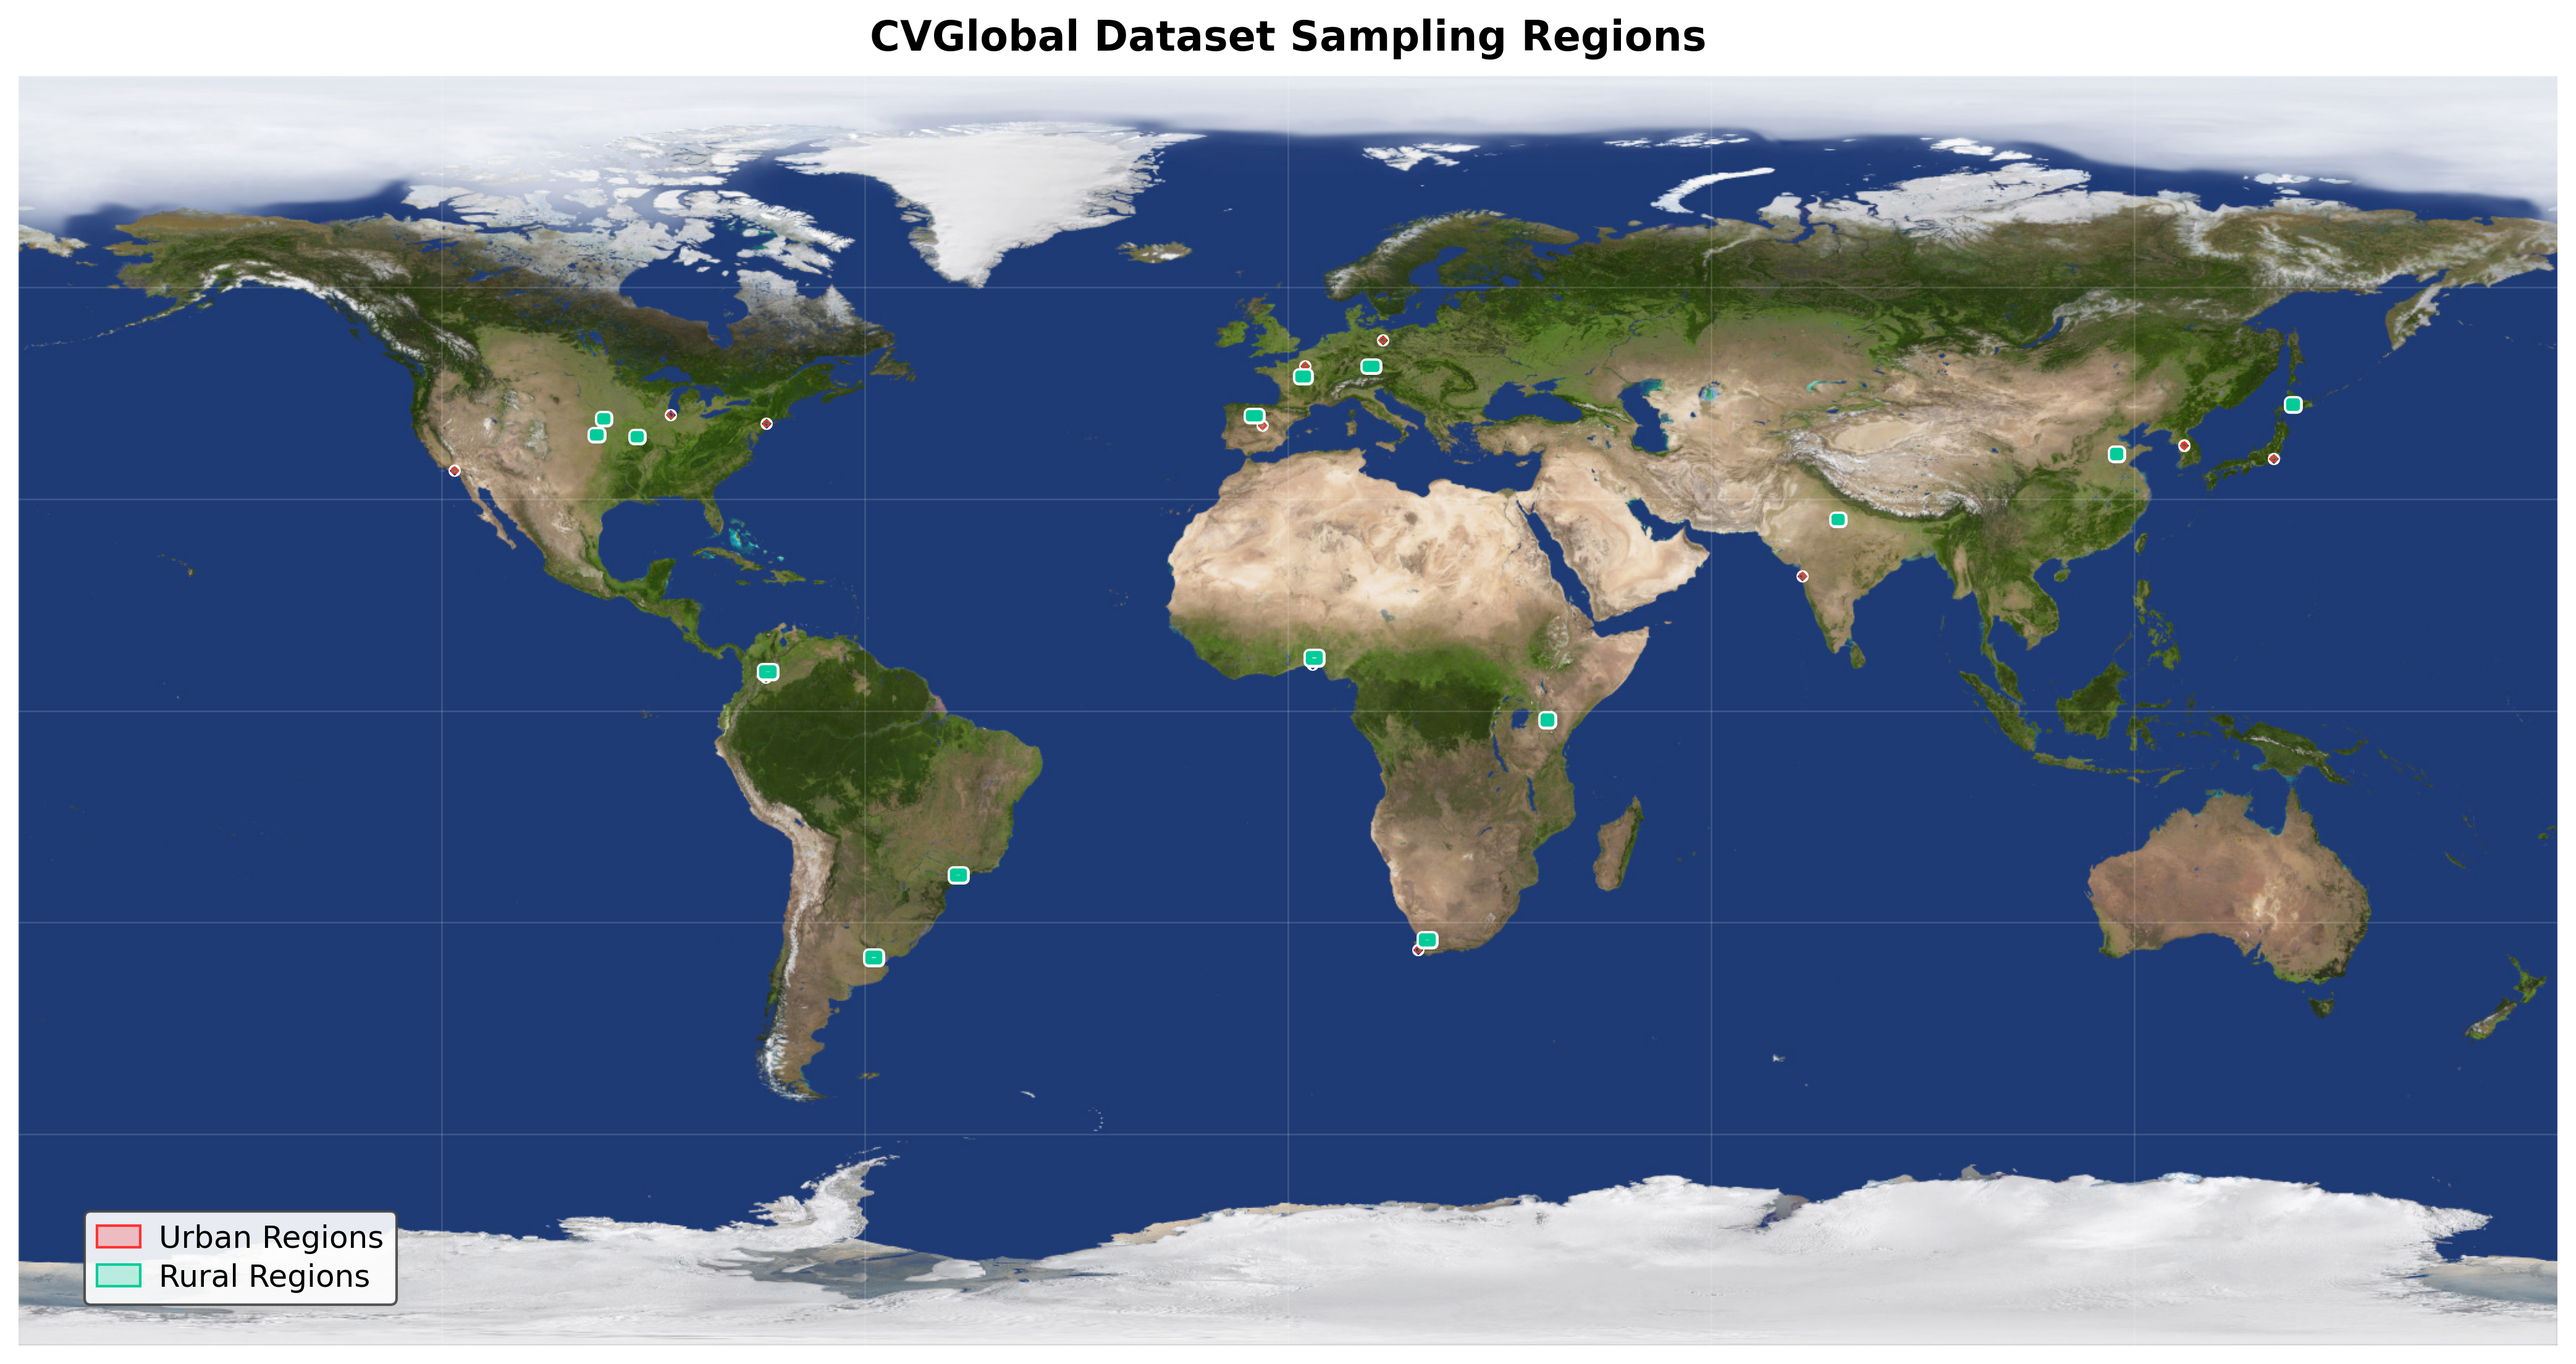
\includegraphics[width=0.8\textwidth]{.././paper/images/sampling_regions_map.png}
    \caption{Global distribution of CVGlobal dataset sampling regions across five continents, showing urban (red) and rural (teal) areas with numbered locations corresponding to Table~\ref{tab:sampling_regions}.}
    \label{fig:sampling_regions}
\end{figure}

\subsection{Data Acquisition Pipeline}

Our data acquisition pipeline ensures high-quality multi-modal data collection through systematic coordinate generation, validation, and image retrieval. For each sampling region, we generate random coordinates and validate them for Street View availability and outdoor environments using Google Places API filtering to exclude indoor locations such as shopping malls and restaurants.

For each validated coordinate, we acquire satellite imagery (640×640 pixels at zoom level 18) and street-view images from four cardinal directions (0°, 90°, 180°, 270°). The directional images are concatenated to create panoramic representations. Our pipeline implements robust error handling with exponential backoff retry strategies and supports resumption capabilities for interrupted data collection sessions.

The resulting CVGlobal dataset provides balanced, geographically diverse paired satellite and street-view imagery suitable for training and evaluating cross-view methods across varied global contexts.